\chapter{Suggested Approach}
\label{sec:approach}

In this chapter, a new approach for solving the floorplanning problem is introduced and described in more details.

\section{B*-Tree}

Coding is a crucial part of every evolutionary algorithm. It influences the size and the characteristic of the search space, the quality of the solution and the speed of coding and decoding. As the decoding is executed for every iteration, generation and individual, its speed is critical. For example, if we use 1,000 iterations, 500 generations and have population of 100, the coding process may be executed $ 1000 \cdot 500 \cdot 100 = 50,000,000 $ times. If the decoding process takes 1 ms, the total time of 13 hours is reached. Of course, this count can be lowered by evaluating only individuals not already evaluated. But still the coding takes a large amount from the algorithm running time.

Therefore, the B*-Tree representation \cite{btree} was chosen to be used in the suggested algorithm. The B*-Tree is a regular hierarchical structure, allowing effective tree operations (including placing) and providing many options for tree permutation. By altering the B*-Tree nodes, many different floorplans can be created from the original prototype easily. 

As noted in previous chapters, the conversion from the B*-Tree to the placement can be done in amortised linear time using the {\em contour data structure} (or similar), introduced in \cite{otree}. Without this structure, the worst case would be quadratic to the number of modules.

B*-Tree does not differ from the ordinary binary tree, a common data structure, often used in many implementations of sets, priority queues, etc. The only difference is in values it holds. The algorithm will work with B*-Trees of modules, both unplaced and placed.

Also, for doing permutations using the POEMS actions, all B*-Tree nodes must be addressable. So each node in a B*-Tree gets an unique integer number, which is used as its address. Further, for creating new or random POEMS actions, it will be also required to generate random addresses. As an each address is an integer, minimum and maximum values must be known at the creation time. Minimum value is defined as $0$, maximum value as $n-1$, where $n$ is a number of modules in the problem set. To make this solution more generic, a counter class is introduced. It allows tree to be numbered by a `hot potato' algorithm and then the last number used can be easily extracted from the same counter object.

Some examples of B*-Tree encoded floorplans are shown in Fig.~\ref{fig:btreef} and Fig.~\ref{fig:btrees}.

\begin{figure}
\centering
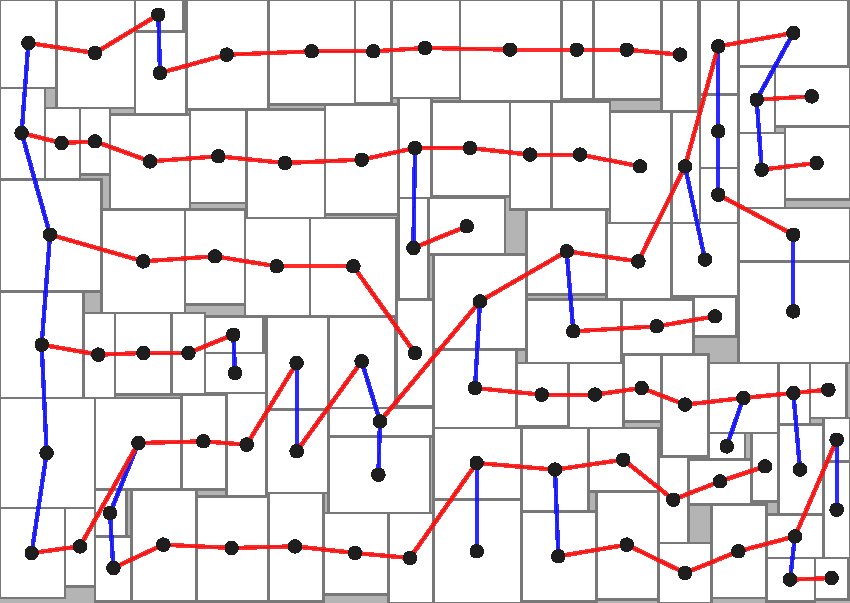
\includegraphics[width=.8\textwidth]{btreebig1}
\caption{An example of a floorplan represented by the B*-Tree}
\label{fig:btreef}
\end{figure}

\begin{figure}
\centering
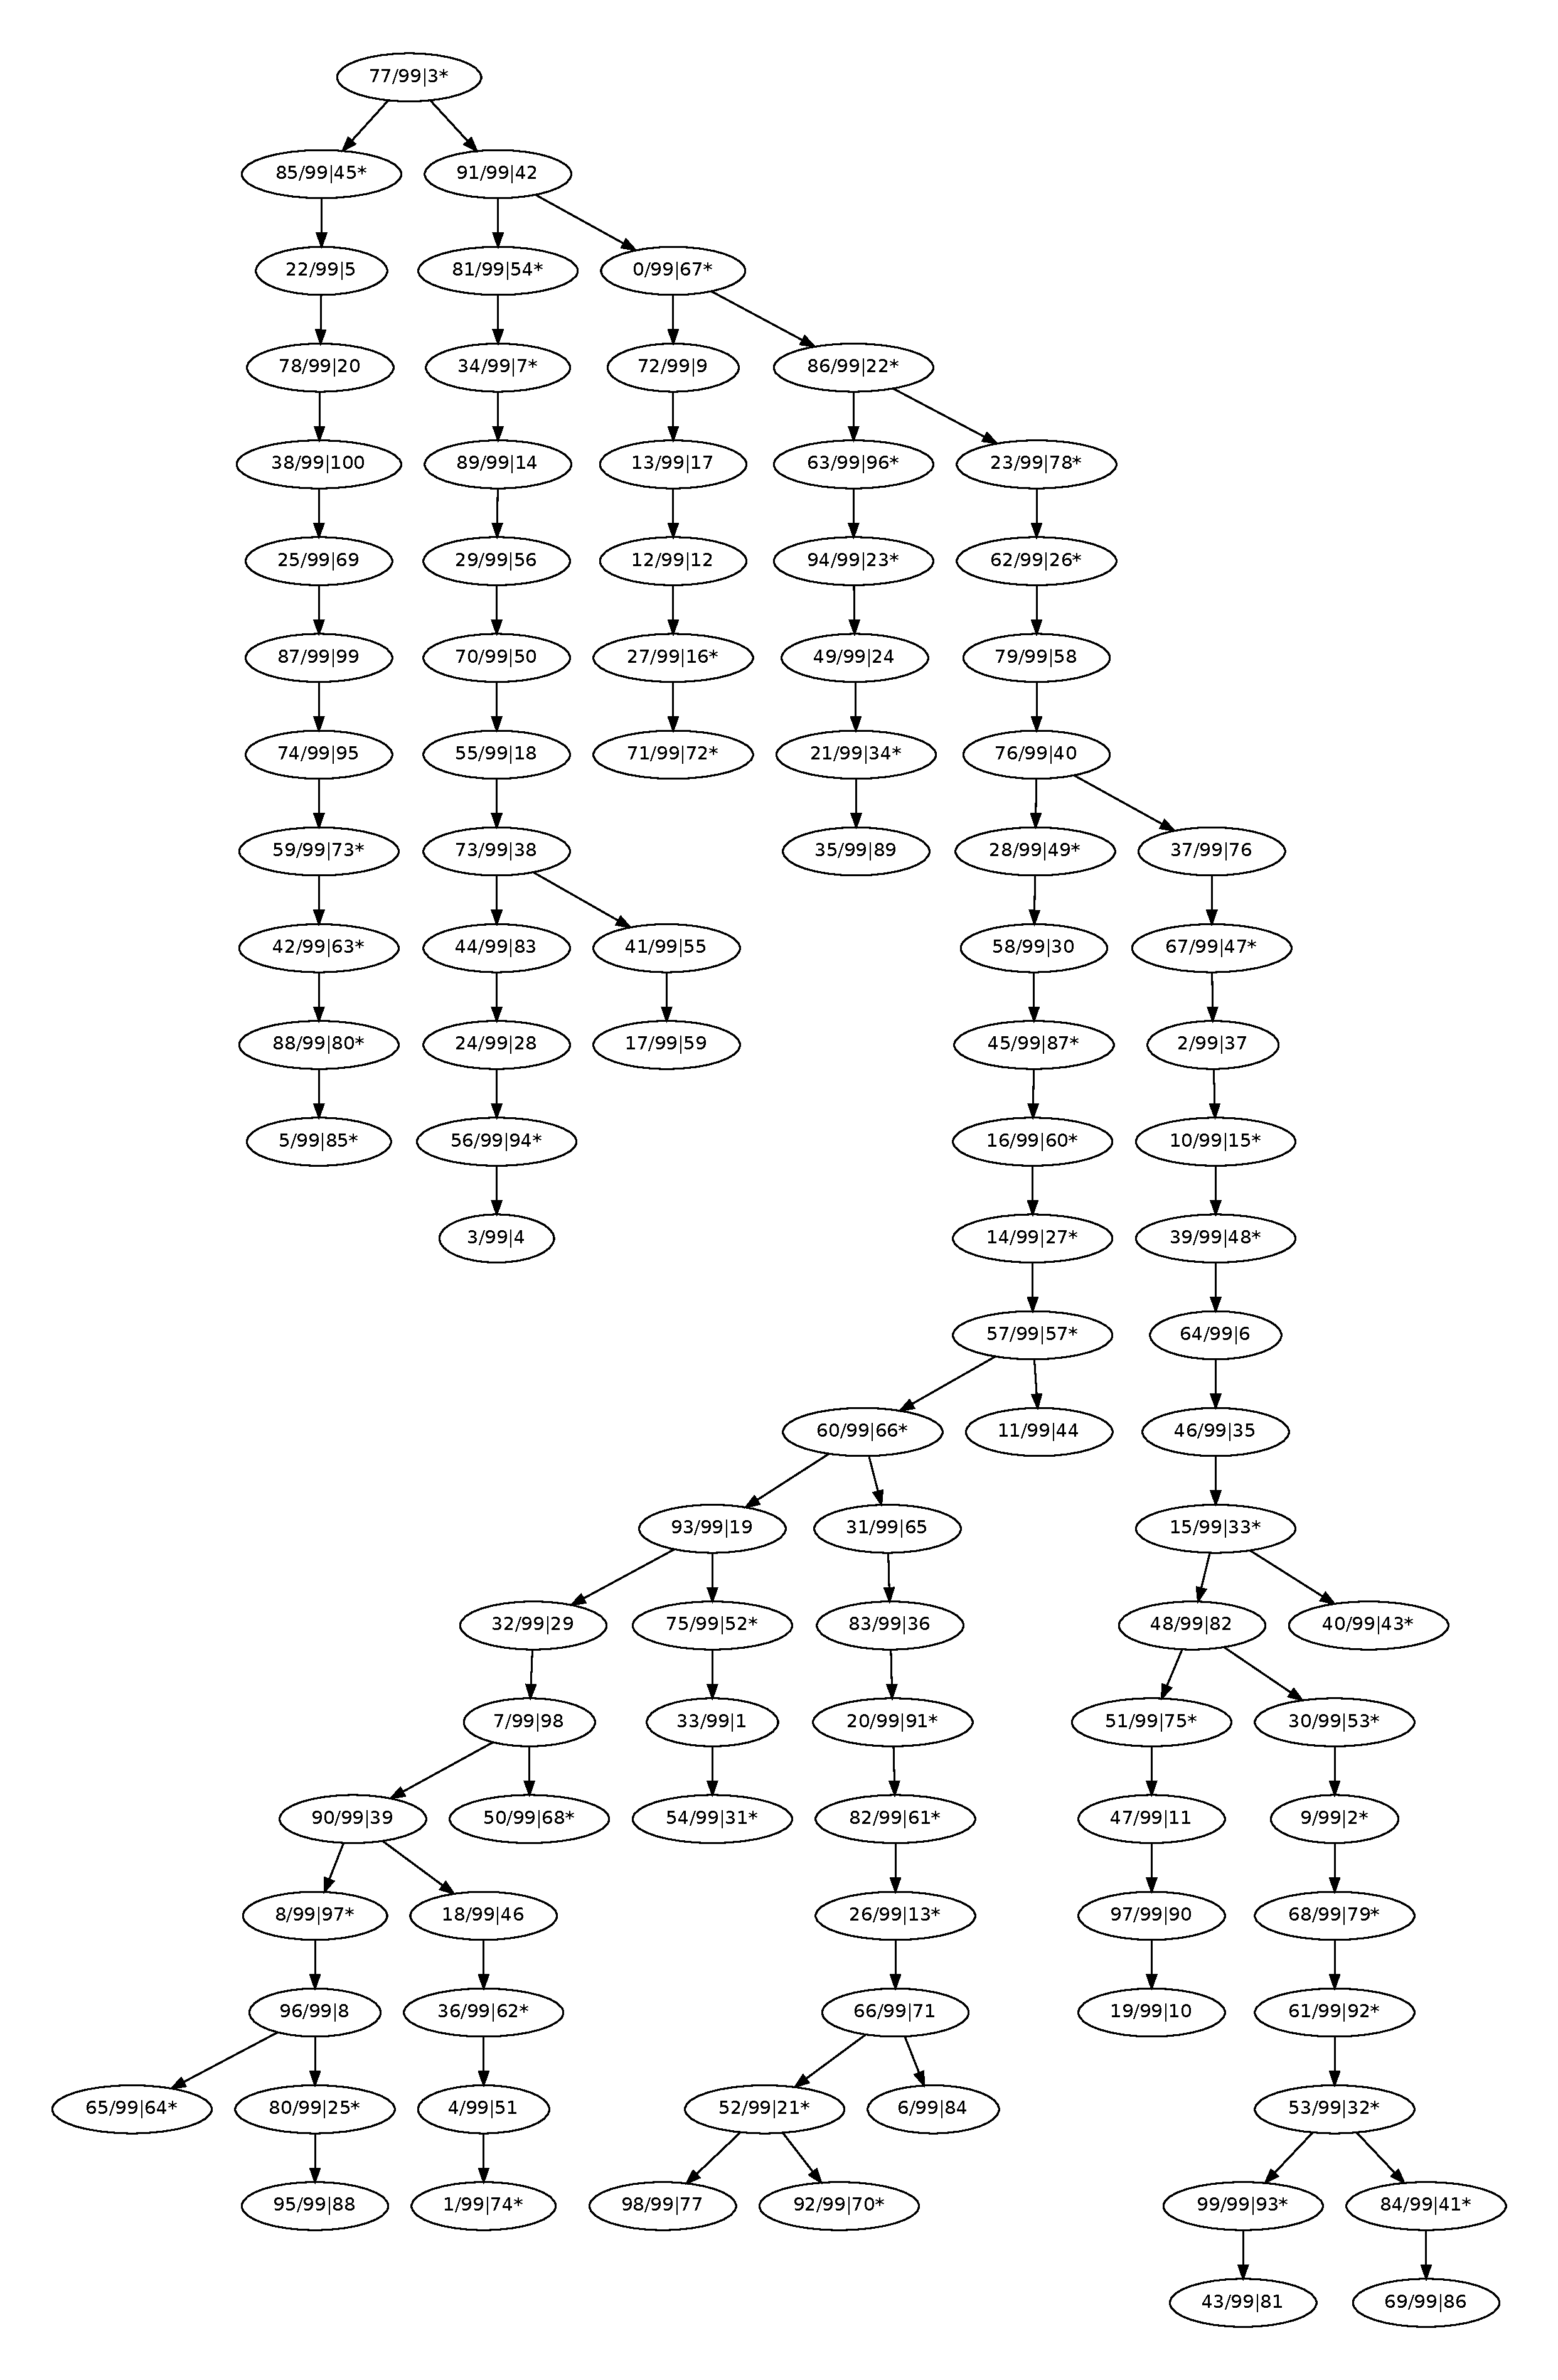
\includegraphics[height=.8\textheight]{btreestruct}
\caption{An example of a floorplan structure represented by the B*-Tree}
\label{fig:btrees}
\end{figure}

\subsection{Placement}

Placement is an assignment of an exact 2D position to each module. In other words, it is a conversion from the B*-Tree of unplaced modules to the B*-Tree of placed modules, which can be done recursively. The root is placed at $(0, 0)$. Then the recursive procedure starts. First, the left subtree of the current node is placed, then the right one.  

When placing the node $i$, the position of its parent $(x_p, y_p)$ is already known. If the node visited is the left child of the parent, its position is defined as $(x_p+w_p, y_i)$, where $y_i$ is the maximal $y$ coordinate of already placed modules which overlap the horizontal interval $(x_p+w_p, x_p+w_p+w_i)$ (quickly obtained by the contour structure). 

If the node visited is the right child of the parent, its position is defined as $(x_p, y_i)$, where $y_i$ is the maximal $y$ coordinate of already placed modules which overlap the horizontal interval $(x_p, x_p+w_i)$ (quickly obtained by the contour structure). 

The helper structure for finding the overlapping modules used in the proposed algorithm (similar to the contour structure) is described in the next chapter.

\subsubsection{Contour helper structure}

The contour structure is used in both \cite{otree} and \cite{btree} to speedup the searching for an $y$ coordinate of the newly- placed module (the other $x$ coordinate is simply given by its parent node). Without this structure, searching would have complexity of $O(n^2)$, where $n$ is the number of modules. It is because all already placed modules must be checked for overlap before placing each module. 

The original contour structure \cite{otree} holds only a subset of already placed modules, which form the `skyline' of the placement. Only these modules must be searched to find the $y$ coordinate of the newly placed module. Usage of the structure is shown in Fig.~\ref{fig:contour}.

In this work, a similar approach is used. Instead of using a doubly linked list of placed modules, the priority queue was used. In this queue, modules are sorted by their top-most $y$ coordinate (descending). Before placing each module, the queue is walked starting from the head until the first module is reached that overlaps with the module being placed. The top-most $y$ coordinate of the module found in the queue is then used as an $y$ coordinate of the newly placed module.

The complexity of this approach should be similar to the original algorithm widely used, it is easier to implement and less error-prone. The performance of the resulting algorithm is evaluated in Table~\ref{tab:placer}.

\section{Evolutionary Algorithms}

\cite{vh} Looking into the world of nature, we can see that a huge number of very difficult problems have been solved since the beginning of the world‘s existence. It was, for example, parts of the body and organs, and their functions in the body. Living creatures have had to learn how to survive in dangerous and changing enviroment. Searching for food, escaping from agressors, raising young ones\ldots these are just several examples of what living beings face and have to solve every day. Life in its richness, all around us, is an evidence that these problems have been and are solved successfully.

It is widely known that the life is based on genetic information (RNA, DNA) and - since the very beginning, the genetic information is being slowly but continuously modified by e.g. radiation or other random physical processes. If a creature whose genetic information was modified grows adult, it can reproduce, preserve and pass their genetic information onto the next generation. In addition, individuals can combine their genomes: hence, higher quality may be created by means of hybridization (crossover). This process, in a long prospective, is called and described as {\em evolution}.

The mankind is an integral part of the nature, and draws inspiration from the nature every day - in music, art, construction, and in problem-solving as well. Using modern computer technology, it is possible to simulate the ways in which the nature faces various challenges and use them for solving real world problems.

The scientific branch that deals with research in natural ways of problem-solving and simulates these processes with use of computers is called {\em soft-computing}. This branch has existed for decades and it has already influenced various areas of computer technology and cybernetics. Because of continuous development and progress in this field, we can use and enjoy numerous achievements of modern technology. The already mentioned simulated evolutionary processes are called {\em evolutionary algorithms} - as they, in fact, may simulate the evolution. The main purpose of them is a search for an optimal solution for a particular problem.

The subject-matter of this work is the application of the {\em POEMS} iterative optimisation framework \cite{poems} and the {\em genetic algorithm} to the 2D rectangle packing problem (also known as {\em floorplanning}). This optimisation problem is NP-hard and suitable for evolutionary algorithms.

Evolutionary algorithms are inspired by on evolutionary processes in the nature. They are popular and widespread, as they are easily grasped even by novice researchers and programmers, but they do not guarantee good results in all scenarios automatically. The key \cite{hynek} is to use as much knowledge about the concrete problem as possible or combine the evolutionary algorithms with the traditional approaches (the process is called {\em hybridization}).

\subsection{Advantages}

\begin{itemize}
\item{The algorithms may be customized in order to solve a difficult problem without even knowing its semantics. This is useful for NP-complete problems where no efficient algorithm is known or does not exist at all.}
\item{Acceptable solutions are usually found in reasonable time.}
\item{Most of the processes may be easily implemented and may be run efficiently on parallel computers. This leads to performance scalability.}
\item{They are generally easy to understand because they simulate natural processes.}
\end{itemize}

\subsection{Disadvantages}

\begin{itemize}
\item{These algorithms are not exact: therefore, they are not usable for critical applications. One cannot guarantee that the evolutionary algorithm will find the best solution every time the algorithm is started.}
\item{They work mostly on a random basis. Hence, they may produce different results after every execution.}
\item{Sometimes they `get stuck' at a certain sub-optimal solution, and further improvement is hardly found. Nevertheless, computer scientists often come up with evolutionary algorithm modifications that can slow the `get-stuck process' down or even eliminate it.}
\item{Evolutionary algorithms cannot be used as a universal and `magic' method for solving of all problems in the world. Some voices say that the increasing popularity of evolutionary algorithms is for bad - they are afraid that new computer scientists will lose interest in traditional algorithm research.}
\end{itemize}

\subsection{Basic Types}

\begin{itemize}
\item{{\em Genetic Algorithms} are well-known and versatile evolutionary algorithms. They are based on genetics-related ideas. There is a population of individuals and each of them carries one candidate solution encoded in their genomes. In addition, there is an objective quality-measuring function, the fitness function. It expresses how `good' the solution is. The algorithm runs in iterations that are called `generations'. In every generation, a new population is created by selecting best individuals in the old population and combining them. The algorithm iterates until its terminal condition is encountered, and then returns the best individual found as the problem solution. This algorithm is described in more details below.}
\item{{\em Genetic Programming} uses modified genetic algorithms in order to optimise and generate programmes (instead of encoded solutions). A genetic program comprises a tree structure. It is optimised by adding, removing or moving its tree nodes.}
\item{{\em Memetic Algorithm} is a hybrid genetic algorithm, based on memes instead of genes. Unlike genes, mems can adapt themselves over time.}
\item{{\em Cultural Algorithm} is similar to the genetic algorithm: contrary to it, a cultural algorithm contains a knowledge component - population is enriched by a set of `beliefs', that are shared, used and extended by all individuals. Therefore, it is more similar to the real society.}
\end{itemize}

\section{Genetic Algorithm}

The genetic algorithm is one of the best-known evolutionary algorithms. It was first introduced and researched by John Holland \cite{ga}. The method is inspired by Darwin's theory of evolution \cite{darwin} that describes the development of the life as a continuous struggle between living beings and their enviroment. Only the individuals of highest quality are able to adapt to the natural enviroment - hence survive and reproduce. We can simulate the process in the computer, using problems as an enviroment, and their candidate solutions as individuals.

The very first task for a genetic algorithm designer is to find effective coding of the problem solution. Such coding is to maintain all characteristics of each solution and should be simply creeditable by mutation and crossover operators. For a proper function of the algorithm, a good coding is crucial. For optimisation problems, where both feasible (acceptable) and infeasible (unacceptable) solutions are considered, some kind of additional repair operation may be required to convert an infeasible solution to a feasible one.

What we need is an objective quality-measuring function that will tell us how good the particular solutions are. In nature, this function is simply the ability of individual to survive and reproduce. In an evolutionary algorithm, the function is called {\em fitness function}. This function takes the encoded candidate solution as a parameter, and returns a numeric value. This function should return the maximal (or minimal) value for the optimal solution only (providing that it exists).

To simulate the evolution, genetic algorithms work in iterations that are called {\em generations}. First, an initial population is generated. In every following generation, new individuals are created from the current population with use of {\em selection}, {\em crossover} and {\em mutation} operators. These operators come from their real world counterparts.

New individuals are either copied into a new empty population (generational model, Fig.~\ref{fig:ga_pseudocode_dynamic}) or they replace the worst solutions in the current population (steady-state model, see Fig.~\ref{fig:ga_pseudocode_static}).

To summarise the chapter, before the genetic algorithm can be used for solving a problem, we need to specify the following: the effective coding of the solution; the fitness function; the algorithm for creating the initial population; the selection operator(s); the mutation operator(s); the crossover operator(s); and we have to select the algorithm parameters (but they are usually decided at the run time).

\begin{figure}
\centering
\begin{algorithmic}[1]
  \STATE{create an initial population $ P_0 $ (usually random)}
  \STATE{evaluate the fitness of each invidivual in $ P_0 $}
  \FOR{$ g $ in range 1 .. $ g_{max} $}
    \STATE{create a new empty population $ P_g $}
    \STATE{take individuals from $ P_{g - 1} $ using the selection operator and copy them into the new population $ P_g $ either directly or using crossover and mutation operators}
    \STATE{evaluate the fitness of each individual in $ P_g $}
    \STATE{replace the old population $ P_{g - 1} $ by the new population $ P_g $}
  \ENDFOR
  \RETURN{best-ranked individual from $ P_g $}
\end{algorithmic}
\caption{Genetic algorithm pseudocode (generational model)}
\label{fig:ga_pseudocode_dynamic}
\end{figure}

\begin{figure}
\centering
\begin{algorithmic}[1]
  \STATE{create an initial population $ P $ (usually random)}
  \STATE{evaluate fitness of each invidivual in $ P $}
  \FOR{$ g $ in range 1 .. $ g_{max} $}
    \STATE{take individual(s) from $ P $ using selection operator, apply crossover and/or mutation operators, and replace worst individuals in population $ P $ by them}
    \STATE{evaluate fitness of each individual in $ P $}
  \ENDFOR
  \RETURN{best-ranked individual from $ P_g $}
\end{algorithmic}
\caption{The genetic algorithm pseudocode (steady-state model).}
\label{fig:ga_pseudocode_static}
\end{figure}

\subsection{Initial Population}

Every run of a genetic algorithm begins with a creation of an initial population. It is convenient to generate random solutions in order to cover the widest area within the searching space as possible. We can achieve better results or better performance if we generate additional initial solutions in the areas in which we expect the optimal solution to be found.

There is an important parameter of the genetic algorithm, the {\em population size}. If the population size is too low, the algorithm may degenerate, and nothing new will be found. On the other hand, an excessive population may slow the algorithm down and cause that the algorithm is of no use. There is nothing like a universal value: anyway, in most cases, 50--1000 individuals would be enough.

Some implementations use a special operation, called `immigration'. The immigration causes that some parts of the current population can be replaced by new individuals, either random or created by another (parallel) genetic algorithm. Parallel genetic algorithms are called `population islands', to resemble the reality of several isolated populations. The exchange of individuals between these islands can increases the population diversity.

\subsection{Solution Coding}

The solution coding is the way how the solutions are represented in individual's chromosome. This is probably the most important part of a genetic algorithm. A single problem may be encoded in various ways, and efficient coding is the key to its successful solution. When a genetic algorithm fails, the mistake often is the coding. One coding frequently used is the binary string encoding or the tree encoding.

Binary string encoding is often used for numbers or array of numbers. Numbers are mostly not represented directly, but in a better suited coding, such is the Gray code. If a bit changes in Gray code (e.g. by a mutation operator), the number it represents alters only a little. In a direct representation, MSB flip means much bigger change than flipping LSB. On the other hand, trees represent expressions or computer programs (e.g. in genetic programming, see~\cite{koza}), or other recursive structures. Trees are often encoded as strings using prefix of postfix coding, as i t does not need brackets to retain parenthesis.

\subsection{Fitness Function}

The fitness function, which may be defined for every chromosome, is used for evaluation of the solution quality. The function usually returns non-negative real values: the greater the value is, the better the solution, so the best solution is simply the one with the greatest fitness value. The purpose of the genetic algorithm is to find a solution with the greatest fitness value possible using available operators and in the given time or resource contraints.

There is a simple way to include more parameters in the fitness function: the form $ f(s) = \sum_{\forall i} w_i \cdot X_i \; \; (\sum_{\forall i} |w_i| = 1, |w_i| \in \langle 0,1 \rangle) $, where $ w_i $ is a real number expressing `importance' or `weight' of the input parameter $ X_i $. If we set zero as the weight, the parameter will not be optimised. Alternatively, we can set negative numbers as the weight, if we want to minimise the parameter value.

\subsection{Selection Operator}

In every generation, we can either select certain number of couples and create offsprings by means of crossover operators, or just select sufficient amount of some individuals to clone themselves into a new generation. If we really want to simulate evolution, we must prefer `better' solutions over `worse' ones. That is, the individuals with greater value of the fitness function. There are many ways to accomplish that selection and they are called {\em selection operators}. Some kinds of selection operators are described below.

\subsubsection{Roulette Selection}

Roulette selection is one of the most common algorithms for selection. Every individual is selected with probability according to its relative fitness. There are more variants of the algorithm, because the basic one fails in certain scenarios. The algorithm is based on cumulative fitness and a random threshold that must be satisfied.

\subsubsection{Tournament Selection}

Another simple and widely used type of selection operator is the tournament selection. This algorithm is inspired by struggle between two or more animals for survival. It is obvious, that the `better' animal with higher fitness defeats its enemy, survives and can reproduce itself into another generation. In \cite{tournament} an improvement is suggested, that the better individual should not win always, but only in cca 95\% cases. General algorithm description can be found on Fig.~\ref{fig:tournament}.

\begin{figure}
\centering
\begin{algorithmic}[1]
  \STATE{take $ N $ random individuals from the population}
  \IF{random real number $ \in \langle 0, 1) < 0.95 $}
    \RETURN{individual with the best fitness}
  \ELSE
    \RETURN{random individual}
  \ENDIF
\end{algorithmic}
\caption{The tournament selection algorithm pseudocode}
\label{fig:tournament}
\end{figure}

\subsubsection{Elitism}

There is another good idea in genetics algorithms, the {\em elitism}. The $ N $ best ranked individuals are always copied into the new generation as they are, without any change at all. It prevents the best solution from disappearing from the population.

\subsection{Crossover Operator}

The crossover operator is used in order to combine two or more individuals to produce a new, desirably better ones. The means of the combination may be very simple, for example, splitting parents and then mixing the parts together to create two hybrid descendants. The aim of the crossover is to select best features from both parents, and retain their good attributes into the following generation with the chance of creating even better genome when combining ones. Normally, we do not know which part of parent is the best - so we simply let the crossover happen with certain probability and see if the offspring survives over time. Nevertheless, even `bad‘ descendants may contribute in the process of the search for the optimal solution - since they increase the population diversity. An example of a crossover process is shown in Fig.~\ref{fig:crossover}.

\begin{figure}
\begin{center}
$ \Box \Box \Box \Box \Box \Box \; + \; \blacksquare \blacksquare \blacksquare \blacksquare \blacksquare \blacksquare \; \rightarrow \; \Box \blacksquare \blacksquare \Box \Box \blacksquare $
\end{center}
\caption{The crossover in genetic algorithm}
\label{fig:crossover}
\end{figure}

\subsection{Mutation operators}

The mutation is usually a slight change in individual genetic information. It is caused mainly by radiation or other random physical or chemical processes. The mutation is an engine of the evolution because it often finds an unexpected improvement of current solutions. On the other hand, the mutation may be harmful because it may damage a good individual, too. Some experts say that the mutation is a key part of the genetic algorithm while other operators are only tools for spreading good changes found by mutation through the whole population. An example of the mutation is shown in Fig.~\ref{fig:mutation}.

\begin{figure}
\begin{center}
$ \Box \blacksquare \Box \Box \blacksquare \Box \; \rightarrow \; \Box \blacksquare \blacksquare \Box \blacksquare \Box $
\end{center}
\caption{The mutation in the genetic algorithm}
\label{fig:mutation}
\end{figure}

\section{POEMS Algorithm}

A standard genetic algorithm works directly with solutions yet the POEMS approach introduced in \cite{poems} in combination with the genetic algorithm rather evolves solution modifications. This is a promising method that may prevent (in certains situations) the genetic algorithm from getting stuck at a sub-optimal solution.

The POEMS method works in iterations. Before the first iteration, an initial solution is generated. This solution is called a {\em prototype}. The aim of the following iterations of the POEMS algorithm is to find the best modification of the prototype with use of the genetic algorithm, which serves as a modification optimiser. The prototype modifications are obtained by applying {\em sequences} of defined {\em actions} onto the prototype solution. After each iteration, if an improvement is found, the prototype is replaced. 

In every iteration, a steady-state genetic algorithm is executed in order to find the optimal action sequence. First, a population of $N$ random action sequences of length $L$ is created. The sequences are composed of individual actions and their parameters. The evolution is started, and a selection, crossover and mutation operators are used in order to breed the action sequences. The fitness function of each action sequence is defined as a fitness of the prototype solution after being modified by the particular sequence evaluated.

Generally speaking, POEMS is an iterative stochastic algorithm which uses the genetic algorithm (or some other evolutionary algorithm) for doing the local search during each iteration.

\subsection{Prototype}

A prototype is the initial solution created and improved by the POEMS algorithm. Its creation is a very important step, because the initial position highly influences the space searched. As the solutions are binary trees, a way of creating trees from the initial set of modules must be introduced. 

Two ways of prototype creation were introduced - {\em complete tree} heuristic and {\em best-fit} heuristic. For producing significantly better results, the best-fit heuristic was used in final benchmarks.

\begin{figure}
\centering
\subfloat[complete tree]{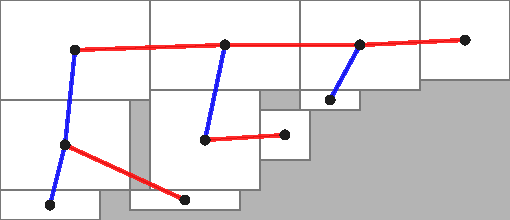
\includegraphics[height=4.5cm]{prototype1}} \hspace{1em}
\subfloat[best-fit heuristic]{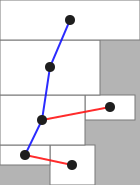
\includegraphics[height=4.5cm]{prototype2}}
\caption{Two ways of creating a prototype example}
\label{fig:prototype}
\end{figure}

\subsubsection{Complete tree heuristic}

The aim of the complete-tree prototype generator is to create a tree as similar to the complete tree as possible. All nodes, except the ones in the last floor, must have exactly two children and must be balanced. 

First, an array of modules is created. The modules are preprocessed by rotation so they are wider than higher. After the rotation, they are sorted by width descending (descending) and height (ascending). Then, the algorithm for creating a heap from an array is used for generating the complete tree from this array of sorted modules.

\subsubsection{Best-fit heuristic}

The best-fit heuristic is a general name for a greedy rectangle packing algorithm. The principle is to select the best fitted module for each hole in the final placement. Both holes and modules are stored in a queue and the algorithm iterates until the module queue is empty. After each placement of the module, the whole list is updated.

A simple heuristic inspired by the best-fit heuristic was introduced to produce accurate prototypes in the suggested floorplan solver. First, it rotates all modules so they are wider than higher and sorts them by width (descending) and height (ascending). This array represents a queue of the modules. 

Then, the tree is built level by level. On each level, a certain limited horizontal space must be filled. Initially, the space to be filled equals to the width of the widest rectangle or the square root of all modules area, whichever is bigger (this is further referred as the {\em original value}). Until the module queue is empty, the algorithm selects the first module from the queue, which can be placed into the space. Then, the module is removed from the queue and the space is shortened by its width. If there is no such module small enough to fit into the space, the current level is ended and a new level is started with the space reset to the original value. 

During this procedure, a tree is being built. The first module placed is marked as the B*-Tree root. The next module in the same level is placed as the left subtree of the previous module and the first module on the next level as the right subtree of the first module in the current level.

\subsection{Actions}

Each action in the POEMS algorithm \cite{poems} represents a certain parameterised modification of the prototype. Individual actions are joined together to sequences that are optimised by the genetic algorithm. 

Every action has a Boolean flag that {\em enables} or {\em disables} the action. If the action is disabled, it does nothing to the input tree. Disabled actions can be used as a special kind of placeholder. \footnote{Disabled actions are somewhere reffered as {\em NOP actions} and enabled actions as {\em active actions}.}

If the enabled and disabled actions were treated equally, the population would be soon infested by disabled actions, because doing nothing to the prototype results in usually better fitness than modifying it somehow. This is the reason for introducing the so called {\em nichés} into the algorithm. Each niché $n$ is a group of individuals that contains only sequences with $n$ or more enabled actions. These nichés are used by the selection operator and during the insertion of the new individual into the population.

Now, the individual action types and their parameters will be introduced.

\subsubsection{Rotate action}

Rotate action flips and mirrors subtrees of every node in the whole subtree starting from the specified tree node. The result is similar to the rotation.

\noindent
\begin{tabular}{|l|l|}
\hline
Parameter 1 & Number of the node to start the rotation from. \\
\hline
\end{tabular}

\subsubsection{Flip action}

Flip action flips (rotates) the module of the specified tree node. If the module is already flipped, it is reverted to its original state.

\noindent
\begin{tabular}{|l|l|}
\hline
Parameter 1 & The number of the node to flip. \\
\hline
Parameter 2 & The action is recursive. \\
\hline
\end{tabular}

\subsubsection{Mirror action}

A mirror action changes the left and the right child of the specified tree node. This action does nothing on the leaf node.

\noindent
\begin{tabular}{|l|l|}
\hline
Parameter 1 & The number of the node whose children will be swapped. \\
\hline
Parameter 2 & The action is recursive. \\
\hline
\end{tabular}

\subsubsection{Exchange value action}

An exchange value action takes two specified nodes and swaps their values. The tree structure is not changed, only the shape of resulting placement is different.

\noindent
\begin{tabular}{|l|l|}
\hline
Parameter 1 & Number of the first node to swap its value. \\
\hline
Parameter 2 & Number of the second node to swap its value. \\
\hline
\end{tabular}

\subsubsection{Exchange node action}

The exchange node action takes the first node specified and inserts it at the position of the second node specified. The second node is placed on the original position of the first node. This operation is permitted only if the first node does not lie in the subtree of the second node and vice versa.

\noindent
\begin{tabular}{|l|l|}
\hline
Parameter 1 & Number of the first node to swap. \\
\hline
Parameter 2 & Number of the second node to swap. \\
\hline
\end{tabular}

\subsubsection{Hang node action}

A hang node action takes the specified source node and places it as the left or the right child of the target node specified. If the target node is located in the subtree starting from the source node, nothing is done. If the target node contains a child at the target position, the child is replaced by the source node and inserted at the original position of the source node.

\noindent
\begin{tabular}{|l|l|}
\hline
Parameter 1 & Number of the source node. \\
\hline
Parameter 2 & Number of the target node. \\
\hline
Parameter 3 & Side to hang on (left or right). \\
\hline
\end{tabular}

\subsection{Genetic Algorithm}

Although various optimisation algorithms can be used in POEMS, the genetic algorithm was chosen. It can be highly customized and the author has some experience with it from previous projects. The steady-state variant was used, because it reaches the convergence quicker.

\subsubsection{Individual and fitness function}

Each individual in the population represents a sequence of actions, which, if applied to the prototype floorplan, creates another floorplan. The fitness function of each individual is computed from the evaluation of the modified floorplan which is created by applying the individual's action sequence to the prototype (each individual gets a reference to the prototype). The fitness value used is the negative amount of the unused area (total area of the enclosing rectangle without the area of placed modules). The relative amount of unused area is computed as (total area $/$ used area) $-1$. Other possibilities include enclosing the rectangle perimeter, the total area or an interconnection volume, which is not considered in this work (but it can be simply added).

The fitness function is assigned the minimal value, in the case the floorplan created by the action sequence is the same as the original one (no changes were made at all). This case may arise when all actions applied cancel their changes mutually. For example, if two flip actions on the same module are done, the result is the same as if there were no flip at all. Removing the obvious useless actions causes the algorithm to search the search space more effectively, forcing it to make bigger steps.

\subsubsection{Population}

The population of the POEMS internal genetic algorithm consist of several groups, numbered from $1$ to $n$. Each group number $n$ can contain only individuals with $n$ or more enabled actions and all groups are the same size. These groups are further referred as {\em nichés}. Population should allow effective searching for individuals from a certain niché. 

\subsubsection{Genetic operators}

The selection operator used in the work is the tournament selection with 2 competitors. First, a random niché is selected. Then, two random competitors within the same niché are picked and compared. The better is returned in 95\% cases, the worse one in 5\% cases \cite{tournament}. Experiments were performed to decide if choosing individuals within the same niché produces better results than choosing both individuals randomly and the results seemed to be slightly better for the first method.

In each generation, new individuals are produced by a crossover or mutation operator (never both at the same time). The crossover algorithm is the uniform crossover, which should perform well on action sequences and is simple to implement. The mutation operator is more complex. Both small (parameter value increments, action order change) and big (parameter value randomization, action sequence shuffle) changes are made. Small changes are occuring more often than big changes. 

Each new individual produced replaces the first individual found, which is of worse or equal fitness and lower or the same niché. If no such individual is found within the population, the new individual is thrown away. This behaviour was introduced, because the algorithm tends to prefer sequences with a lot of disabled actions, as they do not `harm' the prototype. 

\begin{figure}
\centering
\begin{algorithmic}[1]
  \STATE{$n$ = random niché number}
  \STATE{take two random individuals from niché number $n$}
  \IF{random real number $ \in \langle 0, 1) < 0.95 $}
    \RETURN{individual with better fitness}
  \ELSE
    \RETURN{individual with worse fitness}
  \ENDIF
\end{algorithmic}
\caption{The used selection mechanism pseudocode}
\label{fig:tournament}
\end{figure}

\begin{figure}
\centering
\begin{algorithmic}[1]
  \STATE{$c$ = new individual with empty action sequence}
  \FOR{$ i $ in range 0 .. parent 1 sequence length $-1$}
    \IF{random real number $ \in \langle 0, 1) < 0.5 $}
      \STATE{add action at index $i$ from parent 1 to action sequence of $c$}
    \ELSE
      \STATE{add action at index $i$ from parent 2 to action sequence of $c$}
    \ENDIF
  \ENDFOR
  \RETURN{the new individual}
\end{algorithmic}
\caption{The used crossover mechanism pseudocode}
\label{fig:tournament}
\end{figure}
